\documentclass[12pt]{article}
\usepackage{latexblog}

% ============================================================
% Blog Metadata
% ============================================================
\blogtitle{OAuth2授权流程}
\blogdate{2020-09-17}
\blogtags{刨根问底, OAuth, 协议}
\bloglang{zh}
\blogsummary{}

\begin{document}
\makeblogtitle

最近有一个问题一直比较困惑，起因是我们有一个React的应用使用OAuth进行权限验证，而我之前的实践通常是基于Token的权限验证（即通过用户名和密码获取JWT Token），那么OAuth是否适合这样的场景呢？

\section{OAuth 2.0简介}\label{oauth-2.0ux7b80ux4ecb}

\subsection{什么是OAuth}\label{ux4ec0ux4e48ux662foauth}

RFC6749对OAuth 2.0进行了介绍：

\begin{quote}
The OAuth 2.0 authorization framework enables a third-party application to obtain limited access to an HTTP service, either on behalf of a resource owner by orchestrating an approval interaction between the resource owner and the HTTP service, or by allowing the third-party application to obtain access on its own behalf. This specification replaces and obsoletes the OAuth 1.0 protocol described in RFC 5849.
\end{quote}

从这个描述我们可以得出一些结论：

\begin{itemize}
\tightlist
\item
  OAuth 2.0 是一个授权（而不是``认证''）的框架
\item
  OAuth 2.0 设计是为了授权一个第三方的应用访问受限的HTTP服务资源
\item
  OAuth 2.0 出现取代了OAuth 1.0
\end{itemize}

那么，OAuth的出现时为了解决什么问题呢？对于一个典型的客户端请求服务器（受限）资源的场景，譬如一个网络相册服务，客户端需要将用户的认证信息（通常是用户名和密码）发送给服务端，这样才能保证有且仅有这个相册的owner能够访问该相册。现在假设有一个第三方的应用，比如一个什么打印机应用来帮用户打印照片，它也需要调用相册的服务来获取照片，那么显而易见的做法就是将用户的认证信息共享给第三方。但是这样做带来了一些问题：

\begin{itemize}
\tightlist
\item
  第三方应用需要存储用户的认证信息，这样通常是不安全的
\item
  服务器需要能够支持密码认证
\item
  第三方获取到的权限可能比需要要大（比如也许打印机只需要访问一张照片，但是有了用户的认证信息实际上也可以访问到其他的照片，而无法进行限制），而且无法限制其使用时长
\item
  如果期望取消某一个第三方应用的授权，唯一的办法是修改密码，但假设有多个第三方应用那么都会收到影响
\end{itemize}

在OAuth中，客户端通过请求一个单独的access token来访问受限的资源，而token中包含了一些关于权限的描述信息（譬如范围、时效等）。这样在上面的打印照片的例子中，打印服务不需要知道用户的用户名和密码就可以获取到用户想打印的照片。

\subsection{OAuth 中的角色}\label{oauth-ux4e2dux7684ux89d2ux8272}

OAuth中定义了四个角色：

\begin{itemize}
\tightlist
\item
  resource owner：资源所有者（通常是用户），可以授权应用访问其所有的受保护的资源
\item
  resource server：资源服务器，可以根据access token获取受保护的资源
\item
  client：代表resource owner及其授权、访问受保护资源的应用
\item
  authorization server：通过对resource owner认证并获得其授权后，颁发access token的service
\end{itemize}

值得注意的是，这些角色并不要求是分开的实体，同一个server也可以拥有多个角色，例如resource server和authorization server可以是同一个服务。

对于client，又可以分为两种：

\begin{itemize}
\tightlist
\item
  confidential clients: 可以认证的客户端，能够（安全的）保存自身的认证信息
\item
  public clients: 无法存储自身认证信息，例如运行在浏览器或者移动端的应用
\end{itemize}

\section{授权流程}\label{ux6388ux6743ux6d41ux7a0b}

OAuth中最初定义了4种授权方式：

\begin{itemize}
\tightlist
\item
  Authorization Code
\item
  Implicit
\item
  Resource Owner Password Credentials
\item
  Client Credentials
\end{itemize}

后面又发布了一些新的流程和增强，有些已经过时了。

\subsubsection{Authorization Code Grant}\label{authorization-code-grant}

客户端需要生成一个授权链接，包含如下参数：

\begin{itemize}
\tightlist
\item
  response\_type: 必须为\texttt{code}
\item
  client\_id: 客户端标识
\item
  redirect\_uri(Optional): 重定向链接
\item
  scope(Optional): 授权的scope
\item
  state(Recommended): 用来防止跨站请求伪造
\end{itemize}

\begin{Shaded}
\begin{Highlighting}[]
\VariableTok{https}\OperatorTok{://}\VariableTok{authorization}\OperatorTok{{-}}\VariableTok{server}\OperatorTok{.}\VariableTok{com}\OperatorTok{/}\VariableTok{authorize}\NormalTok{?}
  \VariableTok{response\_type}\OperatorTok{=}\VariableTok{code}
  \OperatorTok{\&}\VariableTok{client\_id}\OperatorTok{=}\VariableTok{egHuu4oJxgOLeBzPAQ9sXg4i}
  \OperatorTok{\&}\VariableTok{redirect\_uri}\OperatorTok{=}\VariableTok{https}\OperatorTok{://}\VariableTok{www}\OperatorTok{.}\VariableTok{oauth}\OperatorTok{.}\VariableTok{com}\OperatorTok{/}\VariableTok{playground}\OperatorTok{/}\VariableTok{authorization}\OperatorTok{{-}}\VariableTok{code}\OperatorTok{.}\VariableTok{html}
  \OperatorTok{\&}\VariableTok{scope}\OperatorTok{=}\VariableTok{photo}\OperatorTok{+}\VariableTok{offline\_access}
  \OperatorTok{\&}\VariableTok{state}\OperatorTok{=}\VariableTok{hCi3i1u67XgxqbO}\OperatorTok{{-}}
\end{Highlighting}
\end{Shaded}

授权服务器收到请求后，对请求参数进行检查，如果无误则对用户进行认证，并取得用户授权；授权完成后，授权服务器重定向到请求中的redirect\_uri上，并附加一些参数：

\begin{itemize}
\tightlist
\item
  code: 授权码，必须是在短期内失效（以降低泄漏后带来的风险），建议最长不超过10分钟；客户端对其应该只使用一次，否则授权服务器将拒绝请求并应该尽可能revoke之前通过该code颁发的token。
\item
  state: 即请求中的state值
\end{itemize}

在上面的例子中，当用户授权之后，会跳转到：

\begin{Shaded}
\begin{Highlighting}[]
\VariableTok{https}\OperatorTok{://}\VariableTok{www}\OperatorTok{.}\VariableTok{oauth}\OperatorTok{.}\VariableTok{com}\OperatorTok{/}\VariableTok{playground}\OperatorTok{/}\VariableTok{authorization}\OperatorTok{{-}}\VariableTok{code}\OperatorTok{.}\VariableTok{html}\NormalTok{?}
  \VariableTok{state}\OperatorTok{=}\VariableTok{hCi3i1u67XgxqbO}\OperatorTok{{-}}
  \OperatorTok{\&}\VariableTok{code}\OperatorTok{=}\DecValTok{7}\ErrorTok{RfqR\_w09Ak75fZRlFCVL1ZtKUM3RR67Wd18I9tNZQwSANx9}
\end{Highlighting}
\end{Shaded}

客户端必须首先验证\texttt{state}是否与用户会话中的值一致（这个值可以保存在cookie、session或者通过其他方式保存），从而防止CSRF攻击。验证无误后，客户端需要使用这个code来换取token：

\begin{Shaded}
\begin{Highlighting}[]
\ConstantTok{POST} \VariableTok{https}\OperatorTok{://}\VariableTok{authorization}\OperatorTok{{-}}\VariableTok{server}\OperatorTok{.}\VariableTok{com}\OperatorTok{/}\VariableTok{token}

\VariableTok{grant\_type}\OperatorTok{=}\VariableTok{authorization\_code}
\OperatorTok{\&}\VariableTok{client\_id}\OperatorTok{=}\VariableTok{egHuu4oJxgOLeBzPAQ9sXg4i}
\OperatorTok{\&}\VariableTok{client\_secret}\OperatorTok{=}\VariableTok{p4NlH7i7o2JQJ9xpGdhG95eXWgX1I8teWYZo8pH5}\OperatorTok{{-}}\VariableTok{vILSZXv}
\OperatorTok{\&}\VariableTok{redirect\_uri}\OperatorTok{=}\VariableTok{https}\OperatorTok{://}\VariableTok{www}\OperatorTok{.}\VariableTok{oauth}\OperatorTok{.}\VariableTok{com}\OperatorTok{/}\VariableTok{playground}\OperatorTok{/}\VariableTok{authorization}\OperatorTok{{-}}\VariableTok{code}\OperatorTok{.}\VariableTok{html}
\OperatorTok{\&}\VariableTok{code}\OperatorTok{=}\DecValTok{7}\ErrorTok{RfqR\_w09Ak75fZRlFCVL1ZtKUM3RR67Wd18I9tNZQwSANx9}
\end{Highlighting}
\end{Shaded}

其中：

\begin{itemize}
\tightlist
\item
  grant\_type: 必须为\texttt{authorization\_code}
\item
  code: 上一步从认证服务器拿到的code
\item
  redirect\_uri: 如果拿code这一步有的话这里也必须一致
\item
  client\_id: 客户端标识，如果客户端不是public的话，需要对client进行认证(上面的例子中通过client\_secret进行认证)
\end{itemize}

认证无误后，就可以换取到access\_token了：

\begin{Shaded}
\begin{Highlighting}[]
\FunctionTok{\{}
  \DataTypeTok{"token\_type"}\FunctionTok{:} \StringTok{"Bearer"}\FunctionTok{,}
  \DataTypeTok{"expires\_in"}\FunctionTok{:} \DecValTok{86400}\FunctionTok{,}
  \DataTypeTok{"access\_token"}\FunctionTok{:} \StringTok{"Y80stMYZlsL6p6YSwwR16UiUueaV\_BtuGVVtbmAj{-}b2Y\_5u{-}yKtGqq2gWL2NY6ftKNMo6hin"}\FunctionTok{,}
  \DataTypeTok{"scope"}\FunctionTok{:} \StringTok{"photo offline\_access"}\FunctionTok{,}
  \DataTypeTok{"refresh\_token"}\FunctionTok{:} \StringTok{"eA{-}3mBXx8G9MLDzoKbJZNyV6"}
\FunctionTok{\}}
\end{Highlighting}
\end{Shaded}

\begin{figure}
\centering
\pandocbounded{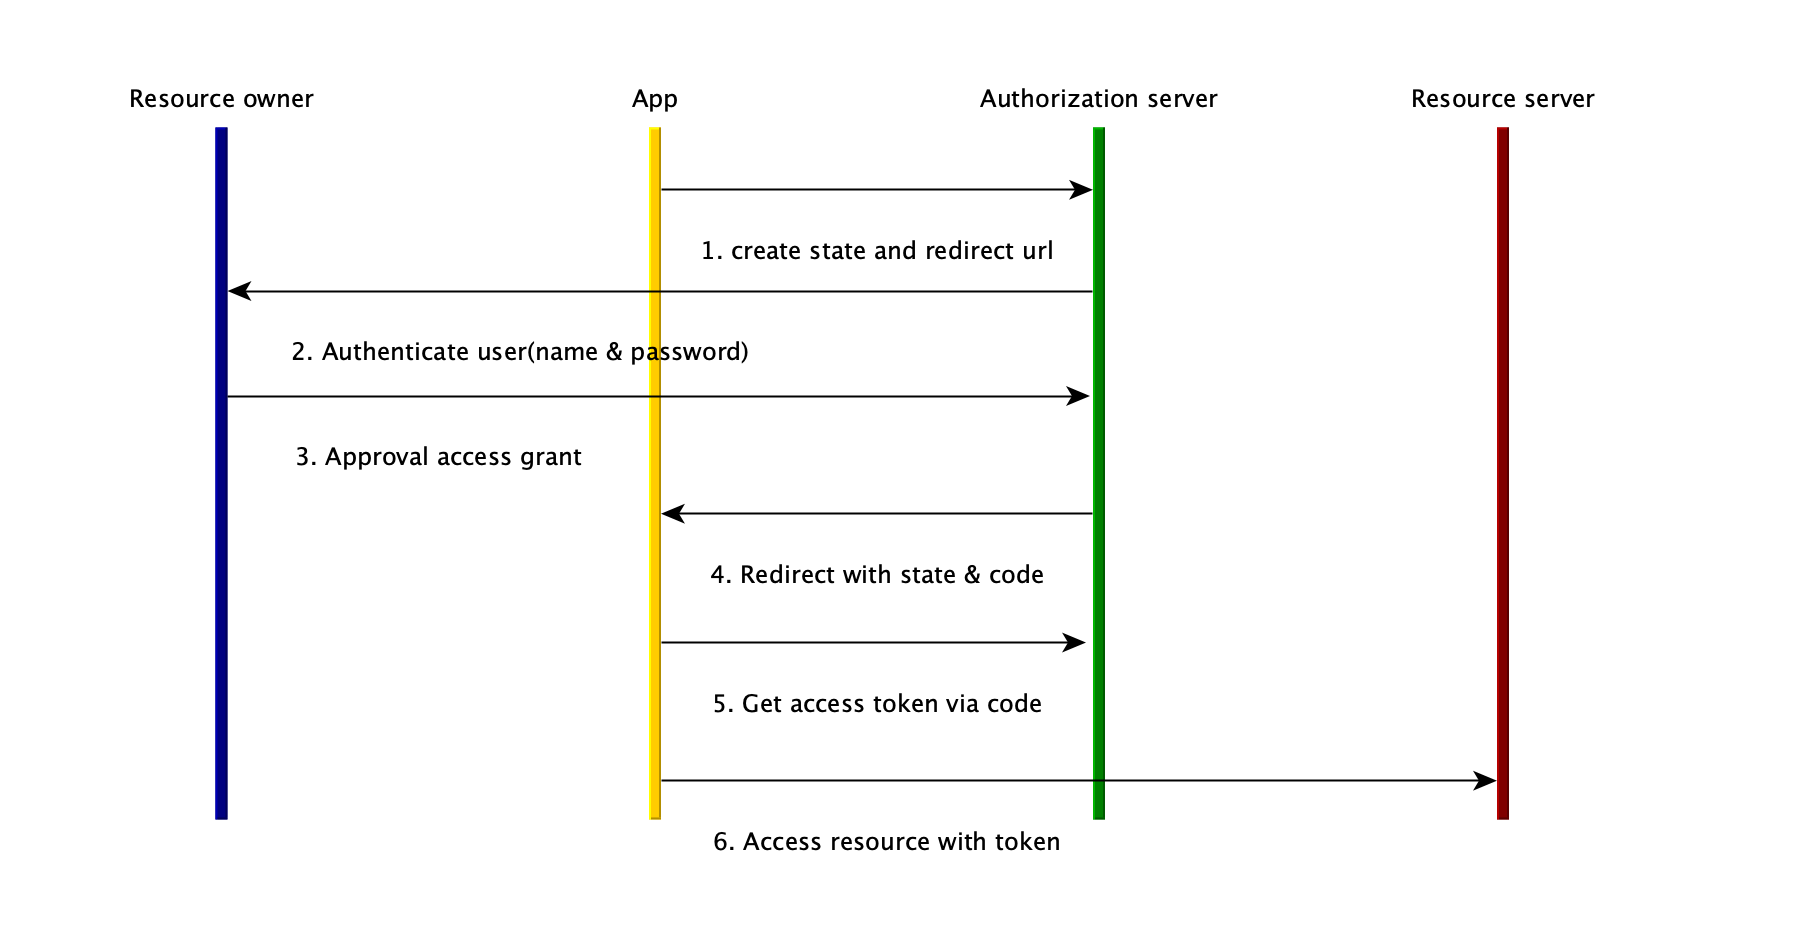
\includegraphics[keepaspectratio,alt={Authrozation code flow}]{images/OAuth-authorization-code-flow.png}}
\caption{Authrozation code flow}
\end{figure}

\subsubsection{Authorization Code Grant with PKCE}\label{authorization-code-grant-with-pkce}

上面一种流程通常推荐跟PKCE（Proof Key for Code Exchange）一起使用来增强安全，区别如下：

\begin{itemize}
\tightlist
\item
  在跳转到authorization server之前，生成一个secret code verifier（43-128位，包含{[}a-zA-Z0-9-.\_\textasciitilde{]}的随机字符串 ）和challenge（通过 \(Base64UrlEncode(SHA256(CodeVerifier))\) 生成）。如果不支持SHA256的话，则跟secret code verifier一致
\item
  challenge在第一次获取code的时候回发送给服务端，服务端会保存challenge；而后在获取access token的时候，客户端需要发送code verifier，从而服务器可以重新进行一次hash来对比
\end{itemize}

例如，

\begin{Shaded}
\begin{Highlighting}[]
\VariableTok{code} \VariableTok{verifier} \OperatorTok{=} \VariableTok{sz3}\OperatorTok{{-}}\VariableTok{THfasVfv882QlbHeLsmBOdkEvgQXAYlce7MTeqzHG7Dk}
\VariableTok{code} \VariableTok{challenge} \OperatorTok{=}\NormalTok{ base64url}\OperatorTok{(}\NormalTok{sha256}\OperatorTok{(}\VariableTok{code\_verifier}\OperatorTok{))} 
               \OperatorTok{=} \VariableTok{pVx7RqTYem8RYTImvRC1M4EsoaOkeqYB6I4l5tnrPWg}
\end{Highlighting}
\end{Shaded}

客户端需要存储code verifier。然后在授权的URL中带上challenge参数：

\begin{Shaded}
\begin{Highlighting}[]
\VariableTok{https}\OperatorTok{://}\VariableTok{authorization}\OperatorTok{{-}}\VariableTok{server}\OperatorTok{.}\VariableTok{com}\OperatorTok{/}\VariableTok{authorize}\NormalTok{?}
  \VariableTok{response\_type}\OperatorTok{=}\VariableTok{code}
  \OperatorTok{\&}\VariableTok{client\_id}\OperatorTok{=}\VariableTok{egHuu4oJxgOLeBzPAQ9sXg4i}
  \OperatorTok{\&}\VariableTok{redirect\_uri}\OperatorTok{=}\VariableTok{https}\OperatorTok{://}\VariableTok{www}\OperatorTok{.}\VariableTok{oauth}\OperatorTok{.}\VariableTok{com}\OperatorTok{/}\VariableTok{playground}\OperatorTok{/}\VariableTok{authorization}\OperatorTok{{-}}\VariableTok{code}\OperatorTok{{-}}\VariableTok{with}\OperatorTok{{-}}\VariableTok{pkce}\OperatorTok{.}\VariableTok{html}
  \OperatorTok{\&}\VariableTok{scope}\OperatorTok{=}\VariableTok{photo}\OperatorTok{+}\VariableTok{offline\_access}
  \OperatorTok{\&}\VariableTok{state}\OperatorTok{=}\VariableTok{G\_SbnGGJEopEPN9A}
  \OperatorTok{\&}\VariableTok{code\_challenge}\OperatorTok{=}\VariableTok{pVx7RqTYem8RYTImvRC1M4EsoaOkeqYB6I4l5tnrPWg}
  \OperatorTok{\&}\VariableTok{code\_challenge\_method}\OperatorTok{=}\ConstantTok{S256}
\end{Highlighting}
\end{Shaded}

同样，授权服务器会重定向到请求的redirect\_uri上并带上state和code

\begin{Shaded}
\begin{Highlighting}[]
\NormalTok{?}\VariableTok{state}\OperatorTok{=}\VariableTok{G\_SbnGGJEopEPN9A}
\OperatorTok{\&}\VariableTok{code}\OperatorTok{=}\VariableTok{dS6}\OperatorTok{{-}}\DecValTok{4}\ErrorTok{QKtIsX6fNBPzxo4DffXTtgufG\_MLbZntG6kQwoEKXUP}
\end{Highlighting}
\end{Shaded}

当客户端拿这个code换取token的时候，需要带上code\_verifier。

\begin{Shaded}
\begin{Highlighting}[]
\ConstantTok{POST} \VariableTok{https}\OperatorTok{://}\VariableTok{authorization}\OperatorTok{{-}}\VariableTok{server}\OperatorTok{.}\VariableTok{com}\OperatorTok{/}\VariableTok{token}

\VariableTok{grant\_type}\OperatorTok{=}\VariableTok{authorization\_code}
\OperatorTok{\&}\VariableTok{client\_id}\OperatorTok{=}\VariableTok{egHuu4oJxgOLeBzPAQ9sXg4i}
\OperatorTok{\&}\VariableTok{client\_secret}\OperatorTok{=}\VariableTok{p4NlH7i7o2JQJ9xpGdhG95eXWgX1I8teWYZo8pH5}\OperatorTok{{-}}\VariableTok{vILSZXv}
\OperatorTok{\&}\VariableTok{redirect\_uri}\OperatorTok{=}\VariableTok{https}\OperatorTok{://}\VariableTok{www}\OperatorTok{.}\VariableTok{oauth}\OperatorTok{.}\VariableTok{com}\OperatorTok{/}\VariableTok{playground}\OperatorTok{/}\VariableTok{authorization}\OperatorTok{{-}}\VariableTok{code}\OperatorTok{{-}}\VariableTok{with}\OperatorTok{{-}}\VariableTok{pkce}\OperatorTok{.}\VariableTok{html}
\OperatorTok{\&}\VariableTok{code}\OperatorTok{=}\VariableTok{dS6}\OperatorTok{{-}}\DecValTok{4}\ErrorTok{QKtIsX6fNBPzxo4DffXTtgufG\_MLbZntG6kQwoEKXUP}
\OperatorTok{\&}\VariableTok{code\_verifier}\OperatorTok{=}\VariableTok{sz3}\OperatorTok{{-}}\VariableTok{THfasVfv882QlbHeLsmBOdkEvgQXAYlce7MTeqzHG7Dk}
\end{Highlighting}
\end{Shaded}

授权服务器会依照这个code\_verifier与之前的challenge进行比较，从而防止有人通过某些途径拿到autorization code之后使用它（因为hash是不可逆的，除非很难通过challenge得到原始的code\_verifier）。

\begin{figure}
\centering
\pandocbounded{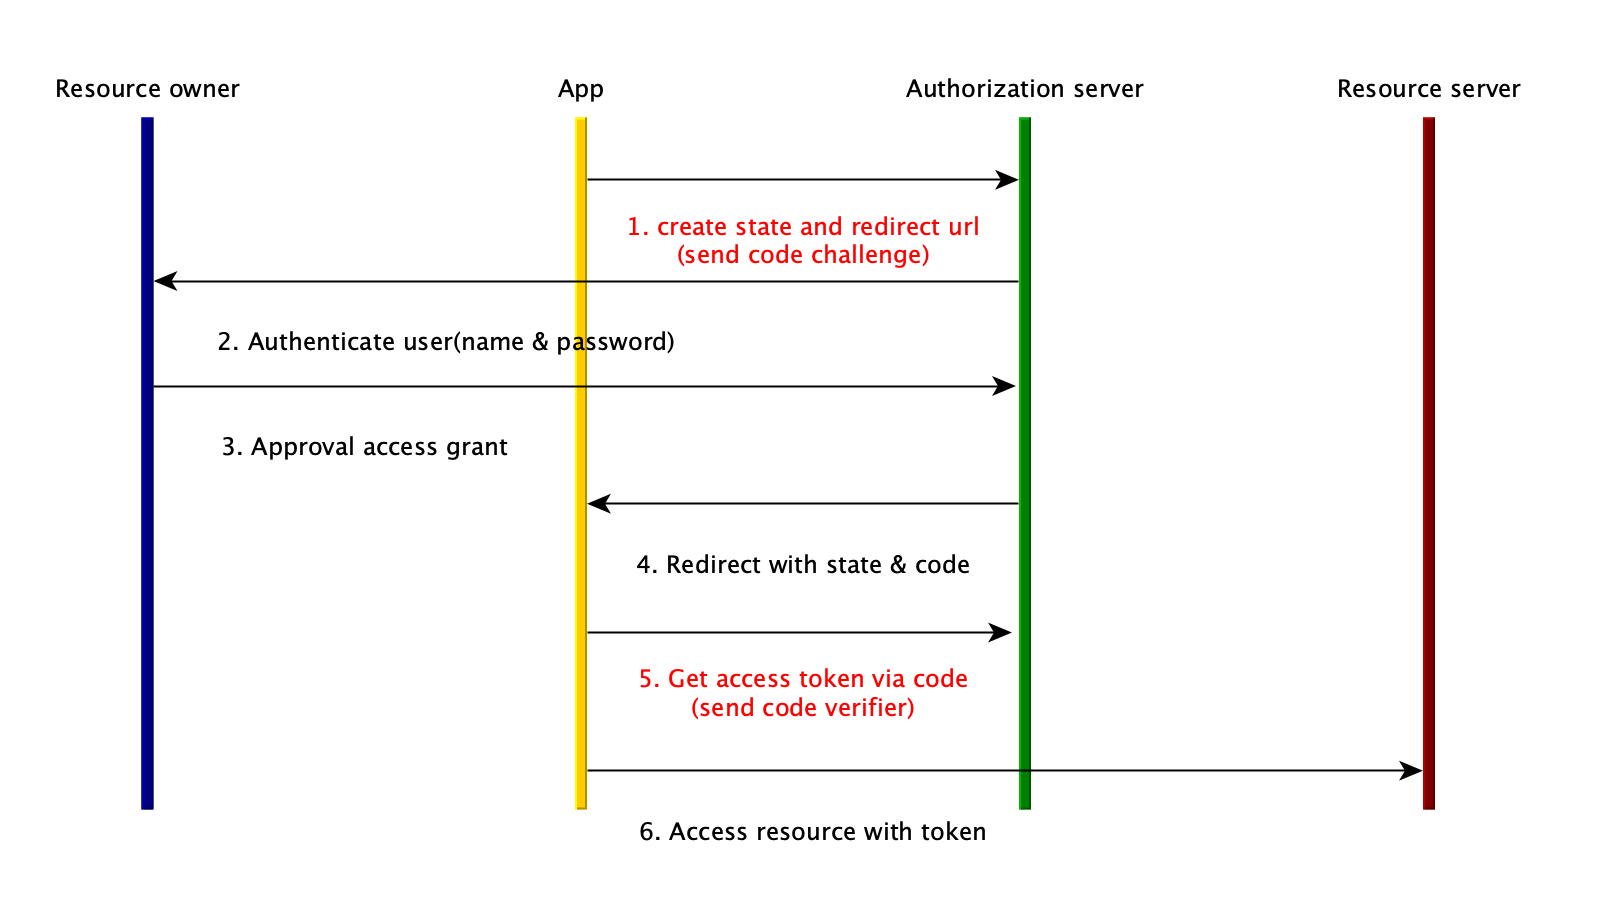
\includegraphics[keepaspectratio,alt={OAuth PKCE}]{images/OAuth-authorization-code-PKCE-flow.png}}
\caption{OAuth PKCE}
\end{figure}

\subsubsection{Legacy: Implicit Grant}\label{legacy-implicit-grant}

首先客户端需要生成一个授权的URL,例如：

\begin{Shaded}
\begin{Highlighting}[]
\VariableTok{https}\OperatorTok{://}\VariableTok{authorization}\OperatorTok{{-}}\VariableTok{server}\OperatorTok{.}\VariableTok{com}\OperatorTok{/}\VariableTok{authorize}\NormalTok{?}
  \VariableTok{response\_type}\OperatorTok{=}\VariableTok{token}
  \OperatorTok{\&}\VariableTok{client\_id}\OperatorTok{=}\VariableTok{egHuu4oJxgOLeBzPAQ9sXg4i}
  \OperatorTok{\&}\VariableTok{redirect\_uri}\OperatorTok{=}\VariableTok{https}\OperatorTok{://}\VariableTok{www}\OperatorTok{.}\VariableTok{oauth}\OperatorTok{.}\VariableTok{com}\OperatorTok{/}\VariableTok{playground}\OperatorTok{/}\VariableTok{implicit}\OperatorTok{.}\VariableTok{html}
  \OperatorTok{\&}\VariableTok{scope}\OperatorTok{=}\VariableTok{photo}
  \OperatorTok{\&}\VariableTok{state}\OperatorTok{=}\VariableTok{wjtEAa38CxUJbhKE}
\end{Highlighting}
\end{Shaded}

其中，response\_type: 必须为token，其他参数与前面的授权流程一样。不同的是，服务端重定向的时候，带的参数为access token而不是code：

\begin{Shaded}
\begin{Highlighting}[]
\OperatorTok{\#}\VariableTok{access\_token}\OperatorTok{=}\VariableTok{cXoSzbih9UYXAZEQlN7gag4sWhvpP9J941OHOhrbXzGqlA\_mzC}\OperatorTok{{-}}\VariableTok{os3u3X4\_g25I1x5epxRM\_}
  \OperatorTok{\&}\VariableTok{token\_type}\OperatorTok{=}\VariableTok{Bearer}
  \OperatorTok{\&}\VariableTok{expires\_in}\OperatorTok{=}\DecValTok{86400}
  \OperatorTok{\&}\VariableTok{scope}\OperatorTok{=}\VariableTok{photos}
  \OperatorTok{\&}\VariableTok{state}\OperatorTok{=}\VariableTok{wjtEAa38CxUJbhKE}
\end{Highlighting}
\end{Shaded}

这种方式虽然简单，但是安全性是比较缺乏的，已经不被推荐使用：

\begin{quote}
It is not recommended to use the implicit flow (and some servers prohibit this flow entirely) due to the inherent risks of returning access tokens in an HTTP redirect without any confirmation that it has been received by the client.
\end{quote}

\begin{quote}
Public clients such as native apps and JavaScript apps should now use the authorization code flow with the PKCE extension instead.
\end{quote}

\subsubsection{Legacy: Resource Owner Password Credentials （Password Grant）}\label{legacy-resource-owner-password-credentials-password-grant}

这种方式即通过用户名和密码来直接获取access token，应用需要将用户的用户名和密码发送给授权服务器来获取token，已经不推荐使用。

\subsubsection{Client Credentials}\label{client-credentials}

将客户端的认证信息作为获取access token的凭证，通常用于访问一些客户端自身的一些资源（而不是用户的资源）。

请求的参数为：

\begin{itemize}
\tightlist
\item
  grant\_type: 为\texttt{client\_credentials}
\item
  scope（Optional)：请求授权的scope
\end{itemize}

例如，一个授权请求：

\begin{Shaded}
\begin{Highlighting}[]
\ConstantTok{POST} \OperatorTok{/}\VariableTok{token} \ConstantTok{HTTP}\OperatorTok{/}\DecValTok{1.1}
     \VariableTok{Host}\OperatorTok{:} \VariableTok{server}\OperatorTok{.}\VariableTok{example}\OperatorTok{.}\VariableTok{com}
     \VariableTok{Authorization}\OperatorTok{:} \VariableTok{Basic} \VariableTok{czZCaGRSa3F0MzpnWDFmQmF0M2JW}
     \VariableTok{Content}\OperatorTok{{-}}\VariableTok{Type}\OperatorTok{:} \VariableTok{application}\OperatorTok{/}\VariableTok{x}\OperatorTok{{-}}\VariableTok{www}\OperatorTok{{-}}\VariableTok{form}\OperatorTok{{-}}\VariableTok{urlencoded}

     \VariableTok{grant\_type}\OperatorTok{=}\VariableTok{client\_credentials}
\end{Highlighting}
\end{Shaded}

这里授权服务器必须要对客户端进行认证（上面的请求中带了客户端的认证信息），如果没有问题则返回token信息：

\begin{Shaded}
\begin{Highlighting}[]
\FunctionTok{\{}
  \DataTypeTok{"access\_token"}\FunctionTok{:}\StringTok{"2YotnFZFEjr1zCsicMWpAA"}\FunctionTok{,}
  \DataTypeTok{"token\_type"}\FunctionTok{:}\StringTok{"example"}\FunctionTok{,}
  \DataTypeTok{"expires\_in"}\FunctionTok{:}\DecValTok{3600}\FunctionTok{,}
  \DataTypeTok{"example\_parameter"}\FunctionTok{:}\StringTok{"example\_value"}
\FunctionTok{\}}
\end{Highlighting}
\end{Shaded}

注意，在这个flow中是不允许包含\texttt{refresh\ token}在返回结果中的。

\subsubsection{Refresh Token}\label{refresh-token}

在前面的流程中，获取access token的同时也会拿到一个refresh token，客户端可以通过这个refresh token来重新拿到一个token。

请求参数：

\begin{itemize}
\tightlist
\item
  grant\_type: 必须为\texttt{refresh\_token}
\item
  refresh\_token: token返回中的refresh token
\item
  scope(Optional): 请求的授权scope，必须是包含在最初拿token时请求的scope中
\end{itemize}

例子：

\begin{Shaded}
\begin{Highlighting}[]
\ConstantTok{POST} \OperatorTok{/}\VariableTok{token} \ConstantTok{HTTP}\OperatorTok{/}\DecValTok{1.1}
     \VariableTok{Host}\OperatorTok{:} \VariableTok{server}\OperatorTok{.}\VariableTok{example}\OperatorTok{.}\VariableTok{com}
     \VariableTok{Authorization}\OperatorTok{:} \VariableTok{Basic} \VariableTok{czZCaGRSa3F0MzpnWDFmQmF0M2JW}
     \VariableTok{Content}\OperatorTok{{-}}\VariableTok{Type}\OperatorTok{:} \VariableTok{application}\OperatorTok{/}\VariableTok{x}\OperatorTok{{-}}\VariableTok{www}\OperatorTok{{-}}\VariableTok{form}\OperatorTok{{-}}\VariableTok{urlencoded}

     \VariableTok{grant\_type}\OperatorTok{=}\VariableTok{refresh\_token}\OperatorTok{\&}\VariableTok{refresh\_token}\OperatorTok{=}\VariableTok{tGzv3JOkF0XG5Qx2TlKWIA}
\end{Highlighting}
\end{Shaded}

服务端必须要对客户端进行认证，并对refresh token进行校验（确保这个refresh\_token有效并且是之前签发给这个client的）。

\subsubsection{Device Code}\label{device-code}

对于无法使用浏览器或者说有输入限制的互联网设备，OAuth 提供了一个Device code的flow。在这个流程中，客户端首先请求一个device code：

\begin{Shaded}
\begin{Highlighting}[]
\ConstantTok{POST} \VariableTok{https}\OperatorTok{://}\VariableTok{example}\OperatorTok{.}\VariableTok{okta}\OperatorTok{.}\VariableTok{com}\OperatorTok{/}\VariableTok{device}

\VariableTok{client\_id}\OperatorTok{=}\VariableTok{https}\OperatorTok{://}\VariableTok{www}\OperatorTok{.}\VariableTok{oauth}\OperatorTok{.}\VariableTok{com}\OperatorTok{/}\VariableTok{playground}\OperatorTok{/}
\end{Highlighting}
\end{Shaded}

然后拿到一个device code:

\begin{Shaded}
\begin{Highlighting}[]
\FunctionTok{\{}
  \DataTypeTok{"device\_code"}\FunctionTok{:} \StringTok{"NGU5OWFiNjQ5YmQwNGY3YTdmZTEyNzQ3YzQ1YSA"}\FunctionTok{,}
  \DataTypeTok{"user\_code"}\FunctionTok{:} \StringTok{"BDWD{-}HQPK"}\FunctionTok{,}
  \DataTypeTok{"verification\_uri"}\FunctionTok{:} \StringTok{"https://example.okta.com/device"}\FunctionTok{,}
  \DataTypeTok{"interval"}\FunctionTok{:} \DecValTok{5}\FunctionTok{,}
  \DataTypeTok{"expires\_in"}\FunctionTok{:} \DecValTok{1800}
\FunctionTok{\}}
\end{Highlighting}
\end{Shaded}

其中的device code和user code是需要展示给用户的。

然后客户端需要一直去poll,

\begin{Shaded}
\begin{Highlighting}[]
\ConstantTok{POST} \VariableTok{https}\OperatorTok{://}\VariableTok{example}\OperatorTok{.}\VariableTok{okta}\OperatorTok{.}\VariableTok{com}\OperatorTok{/}\VariableTok{token}

\VariableTok{grant\_type}\OperatorTok{=}\VariableTok{urn}\OperatorTok{:}\VariableTok{ietf}\OperatorTok{:}\VariableTok{params}\OperatorTok{:}\VariableTok{oauth}\OperatorTok{:}\VariableTok{grant}\OperatorTok{{-}}\FunctionTok{type}\OperatorTok{:}\VariableTok{device\_code}
\OperatorTok{\&}\VariableTok{client\_id}\OperatorTok{=}\VariableTok{https}\OperatorTok{://}\VariableTok{www}\OperatorTok{.}\VariableTok{oauth}\OperatorTok{.}\VariableTok{com}\OperatorTok{/}\VariableTok{playground}\OperatorTok{/}
\OperatorTok{\&}\VariableTok{device\_code}\OperatorTok{=}\VariableTok{NGU5OWFiNjQ5YmQwNGY3YTdmZTEyNzQ3YzQ1YSA}
\end{Highlighting}
\end{Shaded}

当用户完成授权之后，可以得到一个token:

\begin{Shaded}
\begin{Highlighting}[]
\FunctionTok{\{}
  \DataTypeTok{"token\_type"}\FunctionTok{:} \StringTok{"Bearer"}\FunctionTok{,}
  \DataTypeTok{"access\_token"}\FunctionTok{:} \StringTok{"RsT5OjbzRn430zqMLgV3Ia"}\FunctionTok{,}
  \DataTypeTok{"expires\_in"}\FunctionTok{:} \DecValTok{3600}\FunctionTok{,}
  \DataTypeTok{"refresh\_token"}\FunctionTok{:} \StringTok{"b7a3fac6b10e13bb3a276c2aab35e97298a060e0ede5b43ed1f720a8"}
\FunctionTok{\}}
\end{Highlighting}
\end{Shaded}

\section{其他}\label{ux5176ux4ed6}

\subsection{access\_token的验证}\label{access_tokenux7684ux9a8cux8bc1}

当resource server拿到一个access\_token的时候，是需要对其进行验证的，这再RFC7662中已经标准化，可以通过api来进行：

\begin{Shaded}
\begin{Highlighting}[]
\ConstantTok{POST} \OperatorTok{/}\VariableTok{introspect} \ConstantTok{HTTP}\OperatorTok{/}\DecValTok{1.1}
\VariableTok{Host}\OperatorTok{:} \VariableTok{server}\OperatorTok{.}\VariableTok{example}\OperatorTok{.}\VariableTok{com}
\VariableTok{Accept}\OperatorTok{:} \VariableTok{application}\OperatorTok{/}\VariableTok{json}
\VariableTok{Content}\OperatorTok{{-}}\VariableTok{Type}\OperatorTok{:} \VariableTok{application}\OperatorTok{/}\VariableTok{x}\OperatorTok{{-}}\VariableTok{www}\OperatorTok{{-}}\VariableTok{form}\OperatorTok{{-}}\VariableTok{urlencoded}
\VariableTok{Authorization}\OperatorTok{:} \VariableTok{Bearer} \DecValTok{23410913}\OperatorTok{{-}}\VariableTok{abewfq}\DecValTok{.123483}

\VariableTok{token}\OperatorTok{=}\DecValTok{2}\ErrorTok{YotnFZFEjr1zCsicMWpAA}
\end{Highlighting}
\end{Shaded}

返回如下：

\begin{Shaded}
\begin{Highlighting}[]
\FunctionTok{\{}
  \DataTypeTok{"active"}\FunctionTok{:} \KeywordTok{true}\FunctionTok{,}
  \DataTypeTok{"client\_id"}\FunctionTok{:} \StringTok{"l238j323ds{-}23ij4"}\FunctionTok{,}
  \DataTypeTok{"username"}\FunctionTok{:} \StringTok{"jdoe"}\FunctionTok{,}
  \DataTypeTok{"scope"}\FunctionTok{:} \StringTok{"read write dolphin"}\FunctionTok{,}
  \DataTypeTok{"sub"}\FunctionTok{:} \StringTok{"Z5O3upPC88QrAjx00dis"}\FunctionTok{,}
  \DataTypeTok{"aud"}\FunctionTok{:} \StringTok{"https://protected.example.net/resource"}\FunctionTok{,}
  \DataTypeTok{"iss"}\FunctionTok{:} \StringTok{"https://server.example.com/"}\FunctionTok{,}
  \DataTypeTok{"exp"}\FunctionTok{:} \DecValTok{1419356238}\FunctionTok{,}
  \DataTypeTok{"iat"}\FunctionTok{:} \DecValTok{1419350238}\FunctionTok{,}
  \DataTypeTok{"extension\_field"}\FunctionTok{:} \StringTok{"twenty{-}seven"}
\FunctionTok{\}}
\end{Highlighting}
\end{Shaded}

Ref:

\begin{itemize}
\tightlist
\item
  \href{https://tools.ietf.org/html/rfc6749}{RFC6749 - The OAuth 2.0 Authorization Framework}
\item
  \href{https://tools.ietf.org/html/rfc7636}{RFC7636 - PKCE extension}
\item
  \href{https://tools.ietf.org/html/rfc8628}{RFC8628 - OAuth 2.0 Device Authorization Grant}
\item
  \href{https://tools.ietf.org/html/rfc6819}{RFC6819 - OAuth 2.0 Threat Model and Security Considerations}
\item
  \href{https://tools.ietf.org/html/draft-ietf-oauth-jwt-bcp-07}{RFC7519 - JSON Web Token Best Current Practices}
\item
  \href{https://tools.ietf.org/html/rfc7662}{RFC7662 - OAuth 2.0 Token Introspection}
\item
  \href{https://www.oauth.com/playground/}{OAuth 2.0 Playground}
\item
  \href{https://tools.ietf.org/html/draft-ietf-oauth-security-topics-15}{OAuth 2.0 Security Best Current Practice}
\item
  \href{https://oauth.net/articles/authentication/\#common-pitfalls}{Common pitfalls for authentication using OAuth}
\item
  \href{https://stackoverflow.com/questions/40956418/is-oauth2-only-used-when-there-is-a-third-party-authorization}{is oauth2 only used when there is a third party authorization?}
\item
  \href{https://medium.com/securing/what-is-going-on-with-oauth-2-0-and-why-you-should-not-use-it-for-authentication-5f47597b2611}{What is going on with OAuth 2.0? And why you should not use it for authentication.}
\end{itemize}


\end{document}
